%----------------------------------------------------------------------------------------
%	PACKAGES AND DOCUMENT CONFIGURATIONS
%----------------------------------------------------------------------------------------
\documentclass[article, a4paper, 11pt, oneside]{memoir}

% Margins
\usepackage[top=3cm,left=2cm,right=2cm,bottom=3cm]{geometry}

% Encondings
\usepackage[utf8]{inputenc}

% Language
\usepackage[portuguese]{babel}

% Graphics and images
\usepackage{graphicx}
	\graphicspath{{./images/}}

\usepackage{lmodern}        % Latin Modern family of fonts
\usepackage[T1]{fontenc} 

% Listings
\usepackage{listings}
\lstset{language=C}
\usepackage{color}
\definecolor{dkgreen}{rgb}{0,0.6,0}
\definecolor{gray}{rgb}{0.5,0.5,0.5}
\definecolor{mauve}{rgb}{0.58,0,0.82} 

\lstset{frame=tb,
  language=C,
  aboveskip=3mm,
  belowskip=3mm,
  showstringspaces=false,
  columns=flexible,
  basicstyle={\small\ttfamily},
  numbers=none,
  numberstyle=\tiny\color{gray},
  keywordstyle=\color{blue},
  commentstyle=\color{dkgreen},
  stringstyle=\color{mauve},
  breaklines=true,
  breakatwhitespace=true,
  tabsize=3
}

\usepackage{amsmath}

% Color
\usepackage[dvipsnames]{xcolor}

% Tables
\usepackage{tabularx}

% Math symbols
\usepackage{amssymb}

% Paragraph Spacing
\usepackage{parskip}
\usepackage{indentfirst}
\setlength{\parskip}{0.2cm}

% Hyperreferences
\usepackage{hyperref}

% Repeated commands
\usepackage{expl3}
\ExplSyntaxOn
\cs_new_eq:NN \Repeat \prg_replicate:nn
\ExplSyntaxOff

% Header and Footer Things
\usepackage{wallpaper}
\usepackage{fancyhdr}

% Following code to edit the pagestyle
\pagestyle{fancy}
\fancyhf{}
\rhead{RCOM}
\lhead{Redes de Computadores}
\rfoot{Página \thepage}

% Commands
\usepackage{xargs}

%% Linked Email
\newcommand{\email}[1]{
{\texttt{\href{mailto:#1}{#1}} }
}

%----------------------------------------------------------------------------------------
%	DOCUMENT INFORMATION
%----------------------------------------------------------------------------------------
% Title
\title{\Huge \texttt{Redes de Computadores} }
% Authors
\author{
\LARGE \textbf{Turma 1 Grupo 5}\\\\
\begin{tabular}{l r}
	  Diogo Samuel Gonçalves Fernandes	& \email{up201806250@fe.up.pt}\\
	 Paulo Jorge Salgado Marinho Ribeiro  & \email{up201806505@fe.up.pt}\\
\end{tabular}
}

% Date for the report
\date{\today}

% Table of Contents
\addto\captionsportuguese{\renewcommand*\contentsname{Índice}}

%----------------------------------------------------------------------------------------
%	DOCUMENT
%----------------------------------------------------------------------------------------
\begin{document}
%----------------------------------------------------------------------------------------
%	Front Page
%----------------------------------------------------------------------------------------
% Title Author and Date
\maketitle

% More information for front page
\begin{center}
\textbf{Projeto RCOM - 2019/20 - MIEIC}
\Repeat{2}{\linebreak}
\begin{tabular}{l r}
	\textbf{Professor}: 
	\begin{tabular}{l r}
		Rui Campos & \email{rcampos@fe.up.pt}	\\
	\end{tabular}
\end{tabular}
\Repeat{4}{\linebreak}

\end{center}

\newpage
%----------------------------------------------------------------------------------------
%	CHAPTER 1 - Descrição do Problema
%----------------------------------------------------------------------------------------
\chapter[Introdução][Introdução]{Introdução} \label{\thechapter}

Este trabalho consiste no desenvolvimento de uma aplicação de download via ftp e na criação de uma rede. 
O trabalho está portanto, dividido em duas partes distintas:

\begin{itemize}
	\item Parte 1 - Aplicação de download FTP
	\item Parte 2 - Configuração e estudo de uma rede
\end{itemize}

%----------------------------------------------------------------------------------------
%	CHAPTER 2 - Parte 1 - Aplicação de download
%----------------------------------------------------------------------------------------
\chapter[Aplicação de download FTP][Aplicação de download FTP]{Aplicação de download FTP} \label{\thechapter}

A primeira parte deste segundo projeto consiste no desenvolvimento de uma aplicação de download,
que permite transferir um ficheiro de qualquer tipo, de um dado servidor FTP. Após compilar o código
recorrendo ao comando "make", o utilizador deve escrever na consola o seguinte comando, para correr o programa:

./download ftp://[\textless user\textgreater :\textless password\textgreater @]\textless host\textgreater/\textless url-path\textgreater{}

O campo \textless user\textgreater{} deverá conter o username com que o utilizador deseja entrar no servidor, e \textless password\textgreater{} a respetiva password.
No caso de desejar entrar de forma anónima, o utilizador pode introduzir o username "anonymous" e qualquer password ou
pode omitir os campos do \textless user\textgreater :\textless password\textgreater{}, ficando o input na forma:

./download ftp://\textless host\textgreater /\textless url-path\textgreater{}

O campo [host] indicará o endereço do servidor FTP ao qual se deseja conectar, e [url-path] o caminho para o ficheiro que se pretende transferir.

\section{Arquitetura}

A estrutura principal do programa encontra-se bem explícita no ficheiro clientTCP.c.
O programa começa por processar o argumento introduzido pelo utilizador, armazenando o seu username,
password, o host, e o path para o ficheiro, recorrendo à função parseArguments() que se encontra definida no ficheiro utils.c.
Se o input recebido for inválido, o programa termina e é apresentada uma mensagem indicando a correta utilização do programa.

De seguida, é processado o campo host, obtendo-se o endereço IP correspondente, com recurso à função getIP().
Este endereço IP é utilizado logo na conexão ao servidor, após criação de um socket que será utilizado
para troca de comandos entre o cliente e o servidor.

Após conectar este socket ao servidor desejado, é lida a resposta do servidor a qual se espera que contenha o código 220,
que indica que a conexão foi estabelecida e que o servidor espera pelo login de um novo utilizador. 

Assim, o próximo passo será efetuar o login (função login()), que consiste numa troca de mensagens entre o cliente e o servidor,
estabelecida da seguinte forma:

\begin{itemize}
  \item Envio do comando "user [user] newline", em que [user] é o username recebido como input
  \item Receção da resposta ao comando user. Se o primeiro dígito do código recebido for 2, então não é requerida password, e o login é efetuado com sucesso. Se esse dígito for 3, então é necessária uma password, e os próximos passos são efetuados.
  \item Envio do comando "pass [password] newline", em que [password] é a password recebida como input
  \item Receção da resposta ao comando pass. Se o código recebido for 230, então a password foi aceite e o login foi efetuado com sucesso. Caso contrário, o programa termina acusando erro no login.
\end{itemize}

Após sucesso no login, é necessário pedir ao servidor para transferir dados em modo passivo. Isto é efetuado na função activatePassiveMode(), que começa por enviar o comando 
pasv newline para o servidor.
Segue-se uma máquina de estados, que vai receber a resposta do servidor a este comando, e que vai armazenar os valores retornados, 
utilizando-os para calcular a porta para a qual serão enviados os dados. 

Após isto, é efetuada a criação de um novo socket e a sua conexão ao servidor, 
pela porta resultante do passo anterior, de onde serão lidos os dados do ficheiro.

Já com tudo configurado, é efetuada a transferência do ficheiro, na função download\textunderscore file(), que começa por mandar
o comando "retr [path] newline" para pedir o ficheiro desejado. Segue-se a leitura da resposta do servidor face a este comando,
a qual se espera ser o código 150, que indica que o ficheiro está pronto para download e o pedido foi aceite. 
Assim, pode-se começar a ler a informação do ficheiro, do socket aberto para leitura dos dados, e enviar a informação para um ficheiro criado imediatamente antes,
cujo nome é obtido aplicando a função basename() ao path recebido como input. Se não tiver ocorrido nenhum erro durante o processo, é apresentada uma mensagem de sucesso,
que indica que o ficheiro foi transferido. 

Por último, o programa fecha os dois sockets abertos.

\section{Resultados}

O nosso programa foi testado para diversos casos, nomeadamente a utilização de diferentes servidores FTP,
diferentes logins (introdução de username e password e entrada em modo anónimo), e a utilização de diferentes tipos e tamanhos, nos ficheiros transferidos.
Para maior compreensão do processo, são imprimidos na consola todos os passos efetuados, assim como as respetivas respostas do servidor.
Concluímos todos os requisitos desta primeira parte com sucesso, pelo que a aplicação encontra-se totalmente funcional e de acordo com o especificado.

\newpage
%----------------------------------------------------------------------------------------
%	CHAPTER 3 - Parte 2 - Experiencias de rede
%----------------------------------------------------------------------------------------
\chapter[Configuração e estudo de uma rede][Configuração e estudo de uma rede]{Configuração e estudo de uma rede} \label{\thechapter}

\subsection{Experiência 1 - Configurar uma rede IP}

Nesta primeira experiência foi ligado o GNU3 ao GNU64, ligando ambos os GNU ao switch e recorrendo à configuração dos seus endereços IP para que pudessem comunicar entre si. 
\begin{lstlisting}
	# No GNU63
	ifconfig eth0 172.16.60.1/24

	# No GNU64
	ifconfig eth0 172.16.60.254/24
\end{lstlisting} 

Esta conexão foi testada recorrendo ao comando ping, e uma vez que foi recebida resposta foi possível confirmar que a mesma estava bem configurada. 
Através da \textbf{figura 1} é possível verificar que se obteve uma resposta do GNU64 (pacotes número 26 e 28) ao ping efetuado a partir do GNU63
(pacotes números 25 e 27).

É possível verificar também que o primeiro pacote trocado é um pacote do tipo ARP. 
O ARP (Address Resolution Protocol) é um protocolo utilizado para obter o endereço MAC associado
a um dado endereço de IP. Para o envio de uma trama para um dado computador presente na rede, o emissor
necessita do endereço MAC correspondente ao endereço IP de destino. Para isto, é enviado um pacote ARP
em modo Broadcast, que contém esse IP e que espera o retorno do endereço MAC desejado.
Isto pode ser observado na \textbf{figura 1}, em que é enviado um pacote ARP em broadcast.
Além de pacotes ARP, são trocados pacotes do tipo ICMP.

É também possível verificar que os IPs de origem e destino dos pacotes ping são os IPs e MACs do GNU63 e do GNU64, respetivamente no caso das requests.
No caso das replies, o IP e MAC da origem vai pertencer ao GNU64 e o de destino ao GNU63.

A distinção entre tramas Ethernet do tipo ARP, IP ou ICMP pode ser feita analisando o cabeçalho dessa trama, que terá valores distintos conforme o tipo de trama.
Por sua vez, o comprimento das tramas pode ser obtido no wireshark, como consta na \textbf{figura 24}, uma vez que essa informação está também presente no cabeçalho da trama.

Por último, a interface loopback é responsável por realizar o diagnóstico de problemas e testes de conectividade.
É o método mais usado para determinar se um dispositivo está online. Esta interface é responsável pelos pacotes que podem
ser observados nas \textbf{figuras 25 e 26}.


\subsection{Experiência 2 - Implementar duas LAN virtuais num switch}

Nesta experiência, foram criadas duas LANs virtuais, ficando o GNU63 e o GNU64 conectados à VLAN60 e o GNU62 conectado à VLAN61.
O GNU62 uma vez que se vai encontrar numa rede diferente do GNU63 e GNU64 não consegue comunicar com os mesmos.


Para configurar esta rede foi necessário ligar o GNU62 ao switch e posteriormente foi necessário criar as VLANs e atribuir as respetivas portas.
As VLANs foram criadas através do switch sendo utilizado o seguinte comando:
\begin{lstlisting}
	conf t
	vlan <y>
	end
\end{lstlisting} 
Em que \textless y \textgreater{} representa o número da VLAN.

Seguiu-se a configuração das VLANs, onde foi necessário adicionar as portas do switch às respetivas VLANs, recorrendo ao seguinte comandos:
\begin{lstlisting}
	conf t
	interface fastethernet 0/<n>
	switchport mode access
	switchport por access vlan <y>
	end
\end{lstlisting} 
Nesta caso está a ser adicionada a porta \textless n\textgreater{} do switch à vlan\textless y\textgreater{}. No nosso caso, o valor de y foi 60 e 61, 
como mencionado previamente.

Após adicionar as duas VLAN e adicionar respetivas portas a cada uma, 
passam a existir dois domínios de transmissão, sendo que um deles contém o GNU63 e GNU64 e o outro contém o GNU62.

Deste modo, quando é feito ping em modo de broadcast a partir do GNU63, o GNU64 como se encontra na mesma VLAN e portanto no mesmo domínio de transmissão
irá conseguir 
receber esses pacotes como é possível constatar com as \textbf{figuras 4 e 5}, enquanto que o GNU62 não recebe qualquer pacote uma vez que se encontra noutra VLAN.
Da mesma forma, quando é feito ping em modo de broadcast a partir do GNU62, quer o GNU63 e GNU64 não irão receber qualquer pacote, como se pode verificar
nas \textbf{figuras 7 e 8}, uma vez que estes dois se encontram num domínio de transmissão diferente.


\subsection{Experiência 3 - Configurar Router em Linux}

Nesta experiência, o GNU64 foi configurado de modo a funcionar como um router, estabelecendo assim a ligação entre as duas VLANs criadas anteriormente.

Para isto, configurou-se a porta ETH1 do GNU64 com um IP no mesmo domínio que o GNU62. Depois, foi necessário configurar as rotas com o comando <route add>. 
No GNU63 adicionou-se a rota que redireciona os pacotes que têm como destino a VLAN61 para o GNU64, 
e o mesmo foi realizado para o GNU62, em que os pacotes que têm como destino a VLAN60 são redirecionados para o GNU64.
Isto pode ser verificado na \textbf{figura 11} quando a partir do GNU63 foi efetuado o comando para dar ping no GNU62 este obteve resposta, 
indicando que os computadores conseguem comunicar entre si.

É também possível verificar a forma como o GNU64 opera através da análise das \textbf{figuras 12 e 13}. Na \textbf{figura 12} é possível observar o tráfego de 
pacotes através da ETH0, 
que corresponde à VLAN60, enquando que na \textbf{figura 13} é possível observar relativamente aos pacotes que são trocados na ETH1, correspondente à VLAN61. 
Os pacotes recebidos a partir da
ETH0 correspondente à VLAN60 provêm do endereço 172.16.60.1 e têm o destino de 172.16.61.1 são reencaminhados para a ETH1 correspondente à VLAN61
Podemos também realçar que o primeiro pacote trocado é do tipo ARP, uma vez que antes da captura destes logs foram eliminadas as tabelas ARP dos três GNUs e estes pacotes são necessários
para ser possivel a comunicação.

Após isto, torna-se possível realizar ping do GNU63 para o GNU62 e vice-versa, uma vez que os pedidos são encaminhados para o GNU64 e este por sua vez consegue comunicar com os outros dois PCs.

A tabela de forwarding define a forma como uma trama será encaminhada de um switch ou router na rede. Contém o destino da rota, a "gateway", que corresponde 
ao próximo ponto por onde a rota passará,
a máscara (netmask), usada para determinar o ID da rede a partir do endereço IP de destino, 
informações e custo da rota, o número de referências para a rota, 
um contador de pesquisas da rota, e a placa de rede responsável pela gateway.

Sempre que um GNU dá ping a outro e o GNU que recebeu o pedido não conhece o endereço MAC do emissor, é enviado um pacote ARP a pedir esta informação, 
como mostrado na experiência 1, que conterá os endereços dos GNU de origem e de destino.
Os pacotes ICMP observados resultam do comando ping, e tratam-se de pacotes de request e reply, uma vez que, após a configuração desta experiência, 
todos os PCs conseguem comunicar entre si.
No caso de não conseguirem comunicar entre si, seriam enviados pacotes ICMP do tipo Host Unreachable.
Os endereços IP e MAC dos pacotes ICMP são os dos PCs de origem e destino.

\subsection{Experiência 4 - Configurar um Router comercial e implementar NAT}

O principal objetivo desta experiência consiste na configuração do router com NAT.

Para a configuração, foi necessário ligar a entrada FE0 do router ao switch.
A porta a que o router se encontra ligado ao switch tem de pertencer à VLAN61 e tal pode ser efetuado como foi
mencionado no experiência 2, adicionando a porta à respetiva VLAN. Após o router estar ligado à VLAN61, 
é necessário ligar a entrada FE1 do router à primeira entrada da régua 1 (6.1) que irá permitir a ligação à internet.

Foi necessário adicionar rotas estáticas para permitir que a conexão com a internet, quer a conexão com a VLAN60.
Os comandos que permitem a criação destas rotas estáticas são os seguintes:

\begin{lstlisting} 
ip route 0.0.0.0 0.0.0.0 172.16.2.254
ip route 172.16.60.0 255.255.255.0 172.16.61.253
\end{lstlisting} 

Posteriormente foi pedido para ser retirado o redirecionamento ICMP no GNU62 e a remover a rota para o GNU64.
Ao ser feito o ping para o GNU63, os pacotes enviados são direcionados para a rota default do router, sendo posteriormente enviadas para o GNU64 e a partir deste
chega ao GNU63. Neste caso é possível observar como mostra a \textbf{figura 14} que o router vai redirecionar os pacotes que chegam até ele. 

Após adicionar novamente a rota é possível observar que os pacotes vão diretamente para o GNU64 e após esse seguem para o GNU63. 
Tal permite concluir que os pacotes enviados durante esta seguem uma dada rota, no caso de esta já estar definida. 
Caso contrário, estes são direcionados para a rota default do router. 

Foi efetuada uma última experiência que consistia em voltar a ativar o redirecionamento ICMP e remover a rota para o GNU64. 
Ao ser efetuado o comando de ping do GNU62 para o GNU63, o router envia apenas um pacote para o ICMP Redirect. Como o redirecionamento está ativo, o
GNU62 guarda a rota na tabela de reencaminhamento o que permite a este computador estabelecer a ligação com o GNU64. Nesta situação foi observado apenas um 
pacote do ICMP Redirect ao contrário do que acontecia anteriormente como mostra a \textbf{figura 14} em que a cada ping era recebido um ICMP Redirect.

Após estas experiências, quando foi efetuado ping no router a partir do GNU63 verificamos que não foi obtida qualquer resposta pelo que tivemos de 
implementar o NAT (Network Address Translation). 
Para a configuração do NAT foi necessária a configuração da interface interna e externa do router, assim como criar uma lista de acessos, sendo este o motivo
do GNU64 não conseguir ter acesso à internet. Os comandos a serem executados no router podem ser vistos nos anexos deste relatório.

O NAT é uma técnica que consiste em reescrever através da utilização de uma tabela hash, 
os endereços IP que utilizam o router de forma a que
um computador de uma rede privada tenha acesso a uma rede pública e tem como objetivo poupar espaço de endereçamento público.
Resumidamente, permite que as redes privadas que usam endereços IPs não registados se conetem à Internet ou a uma rede pública,
a partir de um único endereço público. 
Desta forma, apenas um endereço IP é exigido e este irá representar todos os computadores da rede local.
 
Após a configuração do NAT foi possível a comunicação com o router como é possível verificar na \textbf{figura 16}.

\subsection{Experiência 5 - DNS}			

Nesta experiência, foi configurado o DNS (Domain Name Service). Trata-se de um sistema hierárquico e distribuído de gestão 
de nomes para computadores, serviços ou qualquer equipamento conectado à
 Internet ou a uma rede privada.
Isto é, é um sistema que traduz os hostnames nos respetivos endereços IP, 
recorrendo a servidores de DNS que contém uma base de dados com esta correspondência entre hostnames e IPs.

Para a sua configuração foi necessário alterar o ficheiro resolv.conf, 
adicionando o nome do servidor de DNS e o seu endereço IP, de acordo com o slide 14 do guião do projeto.

Quando se faz ping a um servidor externo, é enviado um pacote de DNS com o pedido do IP do servidor.
A resposta chega na forma de um outro pacote DNS, que após fazer a conversão, 
devolverá o endereço IP correspondente.
Esta troca de pacotes pode ser observada na \textbf{figura 17}.

\subsection{Experiência 6 - TCP connections}

Esta experiência serviu para observação do comportamento do protocolo TCP, 
recorrendo à aplicação que desenvolvemos na parte 1 deste projeto. 

Através da análise das \textbf{figura 18} é possível verificar que a aplicação estabelece duas conexões TCP - 
uma para troca de comandos entre o cliente e o servidor FTP, 
que trata do transporte do controlo de informação FTP, e outra para a receção dos dados enviados pelo servidor.
Cada conexão FTP subdivide-se em três fases: o estabelecimento da conexão, a troca de dados entre o cliente e servidor, e o encerramento da conexão.
O mecanismo ARQ (Automatic Repeat Request) do TCP (Transmission Control Protocol) é utilizado com o método da janela deslizante, 
e consiste no controlo dos erros que ocorram durante a transmissão dos dados.
Recorre a ACK (Acknowledgement numbers), que estão incluídos nas tramas enviadas pelo recetor, indicando se esta foi 
recebida corretamente, sem quaisquer problemas, e recorre também ao "window size", que indica o domínio de pacotes 
possíveis de ser enviados pelo emissor, e ao "sequence number", que indica o número do pacote a ser enviado.
O TCP usa um mecanismo de controlo de congestão end-to-end. Isto significa que o emissor limita ou aumenta a taxa de 
transferência de dados para conexão em função do congestionamento percebido por ele.
A conexão TCP é composta por diversas variáveis, sendo uma delas a janela de congestionamento, que limitará a taxa de envio de pacotes de um dado emissor TCP.

Foi realizada uma segunda experiência em que a meio de uma transferência de um ficheiro no GNU63, 
era iniciada uma transferência a partir do GNU62. Os gráficos das taxas de transferência
obtidos podem ser visualizados nas \textbf{figuras 21 e 22}, em que a primeira corresponde à transferência no GNU62 e a segunda à transferência no GNU63.
Os gráficos obtidos durante a experiência permitem concluir que no início do primeiro download no GNU63, a taxa de transferência aumentou até atingir um máximo. 
Quando o segundo download no gnu62 foi iniciado, verificou-se que à medida que a taxa de transferência aumentava no GNU62, ocorria uma igual diminuição no GNU63. 
Quando a transferência no GNU63
terminou, foi possível observar que a taxa de transferência do GNU62 aumentou, atingiu um máximo e manteve-se constante até ao final da transferência.
Assim, com o aparecimento de uma segunda conexão TCP, dá-se uma diminuição da taxa de transferência e conclui-se que o fluxo dos dados está de acordo 
com o mecanismo de controlo de congestão, tendo em conta que se observa uma menor taxa de transferência no momento em que a rede estava mais congestionada 
(mais downloads simultâneos).



%----------------------------------------------------------------------------------------
%	CHAPTER 4 - Conclusões
%----------------------------------------------------------------------------------------
\chapter[Conclusões][Conclusões]{Conclusões} \label{\thechapter}

Este segundo projeto da unidade curricular Redes de Computadores teve como objetivo, numa primeira parte, a implementação de uma aplicação de download de ficheiros recorrendo ao protocolo FTP,
e, numa segunda parte, à configuração de uma rede de computadores. Apesar de dificultado pelo reduzido tempo que tivemos para aproveitar o laboratório, devido à situação pandémica que atualmente enfrentamos,
este projeto foi terminado com sucesso, sendo que conseguimos desenvolver todos os aspetos pedidos.
Ao mesmo tempo, interiorizamos conceitos importantes nesta área, e compreendemos os diversos protocolos que foram abordados.

Em suma, conseguimos alcançar todos os nossos objetivos, e conhecemos conceitos dos quais nunca antes tínhamos ouvido falar, mas que utilizávamos com frequência no nosso dia-a-dia.

\newpage
%----------------------------------------------------------------------------------------
%	CHAPTER 5 - Anexos
%----------------------------------------------------------------------------------------
\chapter[Anexos][Anexos]{Anexos} \label{\thechapter}

\section{Anexo I - Imagens de experiências}
\subsection{Experiência 1}

\begin{figure}[h]
	\centering
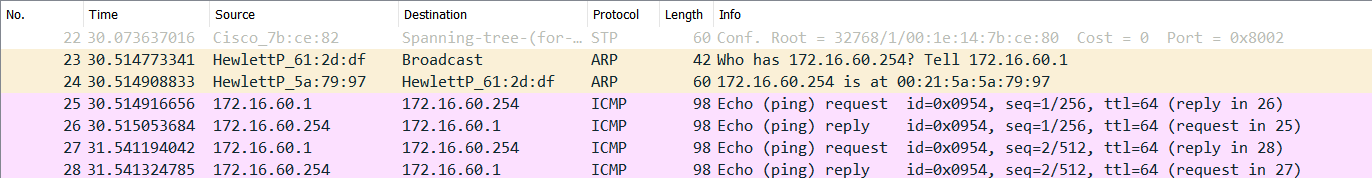
\includegraphics[scale=0.45]{exp1-gnu63.png}
\caption{Ping gnu64 from gnu63}
\end{figure}

\subsection{Experiência 2}
\begin{figure}[h]
	\centering
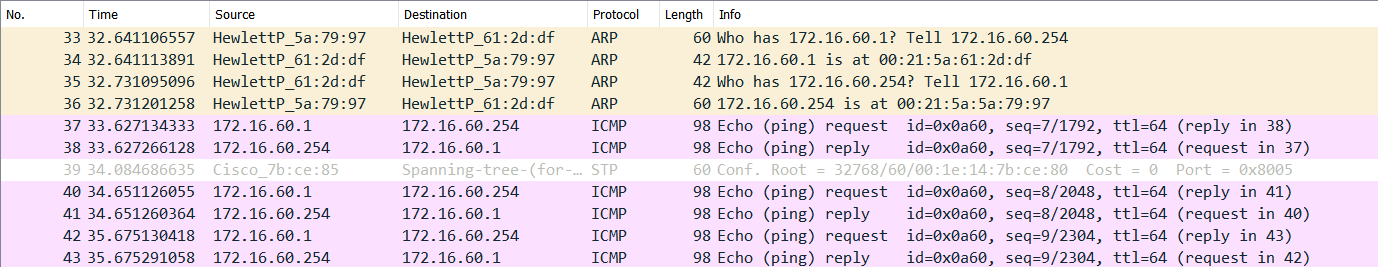
\includegraphics[scale=0.45]{exp2-step5-ping-gnu64-from-gnu63.png}
\caption{Ping gnu64 from gnu63}
\end{figure}

\newpage
\begin{figure}[h]
	\centering
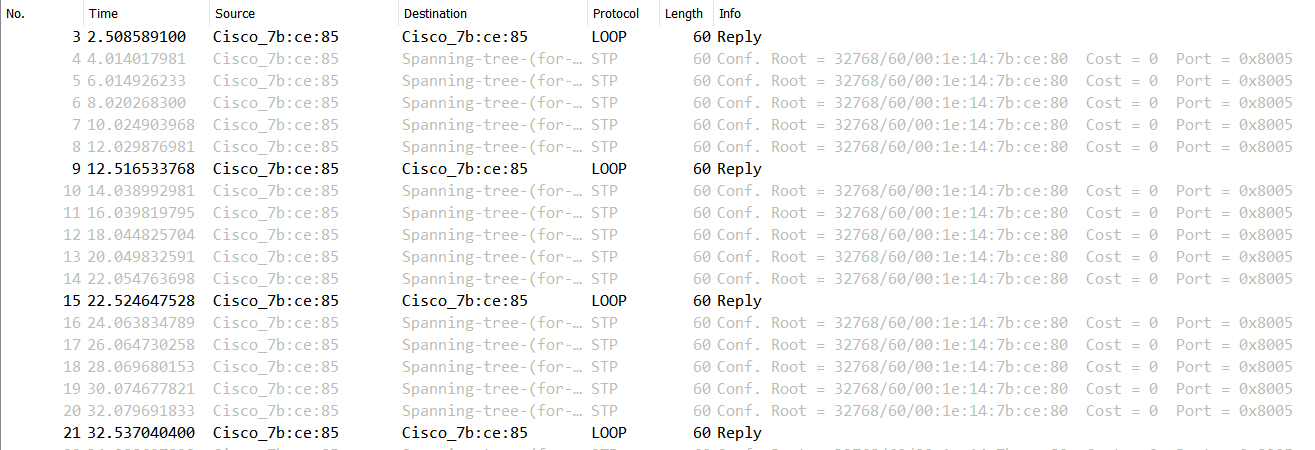
\includegraphics[scale=0.50]{exp2-step8-broadcast-gnu63-from-gnu62.png}
\caption{Ping broadcast a partir do gnu63 (ping –b 172.16.60.255) capturado no gnu62}
\end{figure}


\begin{figure}[h]
	\centering
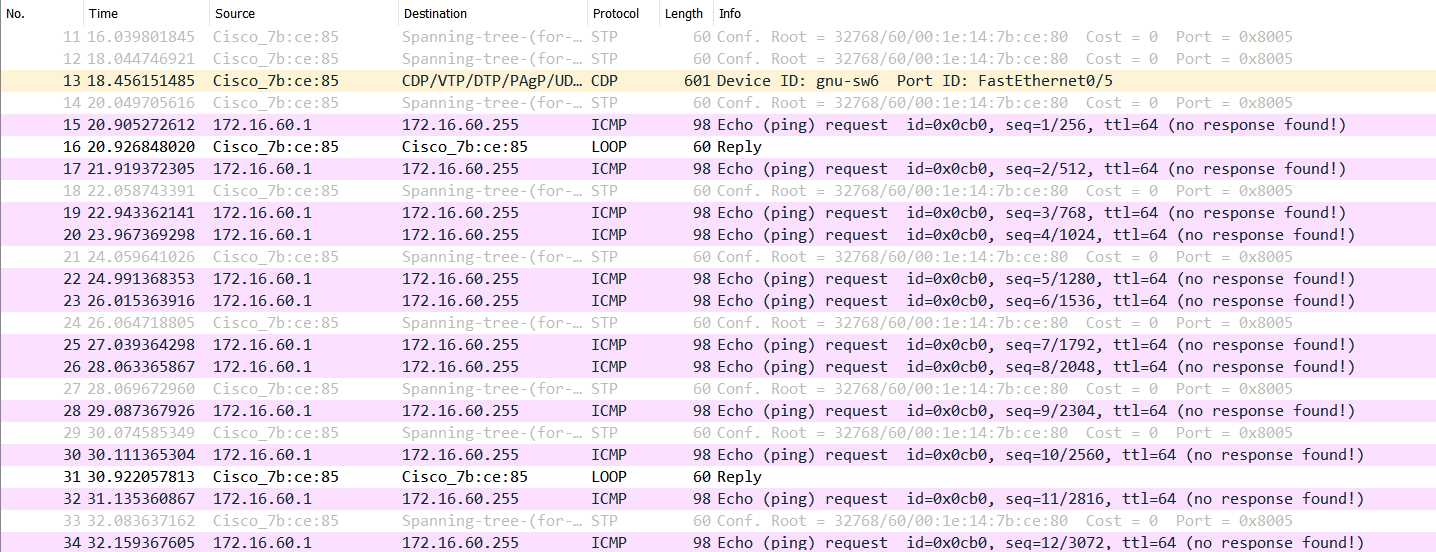
\includegraphics[scale=0.45]{exp2-step8-broadcast-gnu63-from-gnu63.png}
\caption{Ping broadcast a partir do gnu63 (ping –b 172.16.60.255) capturado no gnu63}
\end{figure}

\begin{figure}[h]
	\centering
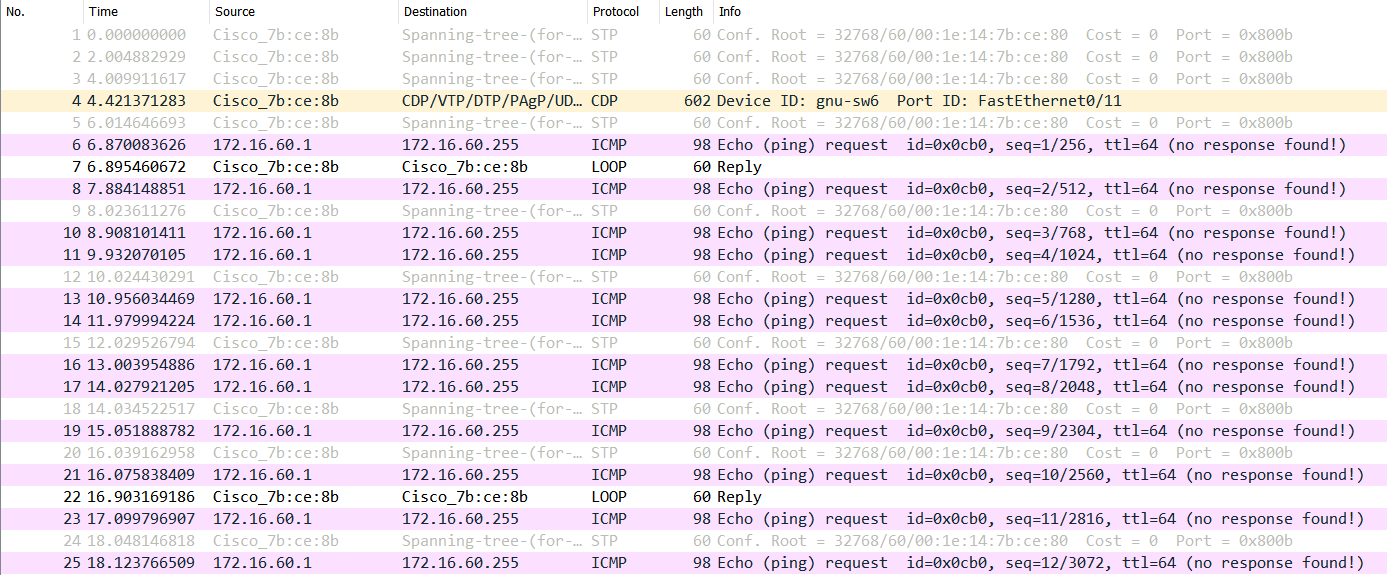
\includegraphics[scale=0.45]{exp2-step8-broadcast-gnu63-from-gnu64.png}
\caption{Ping broadcast a partir do gnu63 (ping –b 172.16.60.255) capturado no gnu64}
\end{figure}

\newpage
\begin{figure}[h]
	\centering
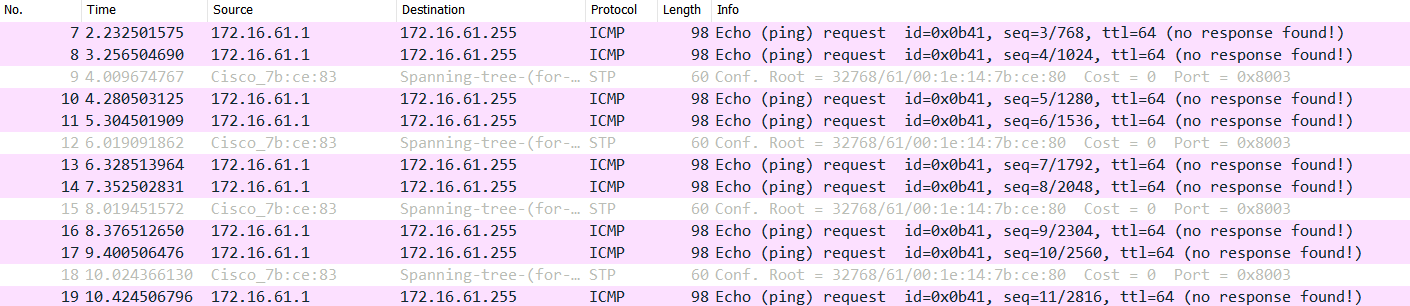
\includegraphics[scale=0.45]{exp2-step10-broadcast-gnu62-from-gnu62.png}
\caption{Ping broadcast a partir do gnu62 (ping –b 172.16.61.255) capturado no gnu62}
\end{figure}


\begin{figure}[h]
	\centering
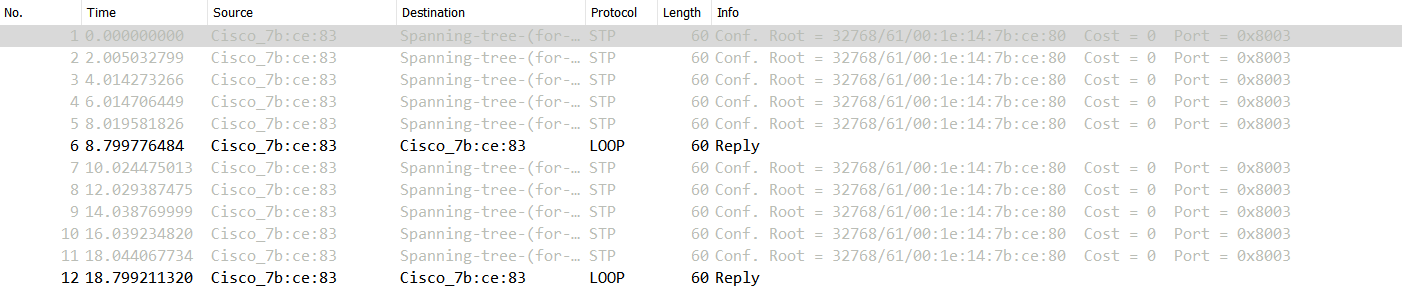
\includegraphics[scale=0.45]{exp2-step10-broadcast-gnu62-from-gnu63.png}
\caption{Ping broadcast a partir do gnu62 (ping –b 172.16.61.255) capturado no gnu63}
\end{figure}

\begin{figure}[h]
	\centering
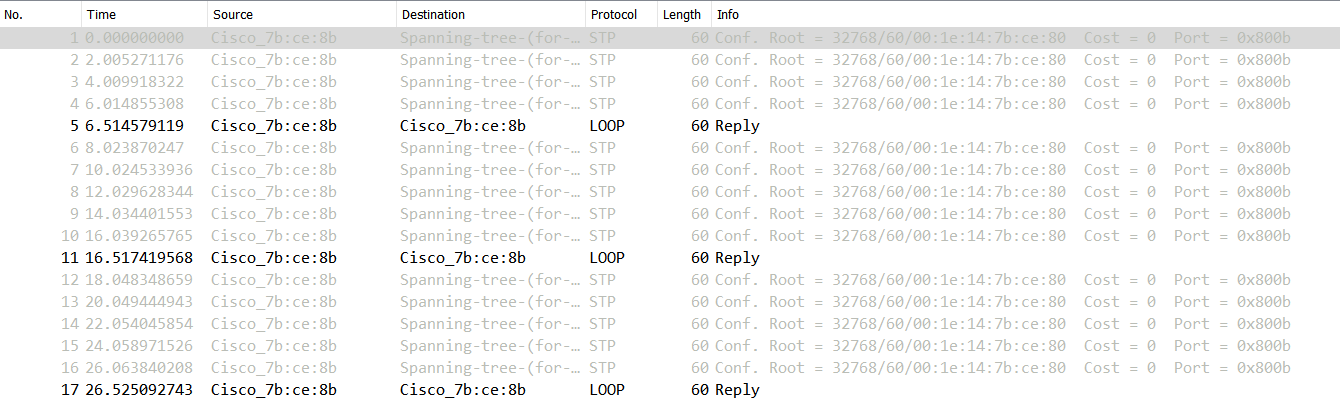
\includegraphics[scale=0.45]{exp2-step10-broadcast-gnu62-from-gnu64.png}
\caption{Ping broadcast a partir do gnu62 (ping –b 172.16.61.255) capturado no gnu64}
\end{figure}

\newpage
\subsection{Experiência 3}
\begin{figure}[h]
	\centering
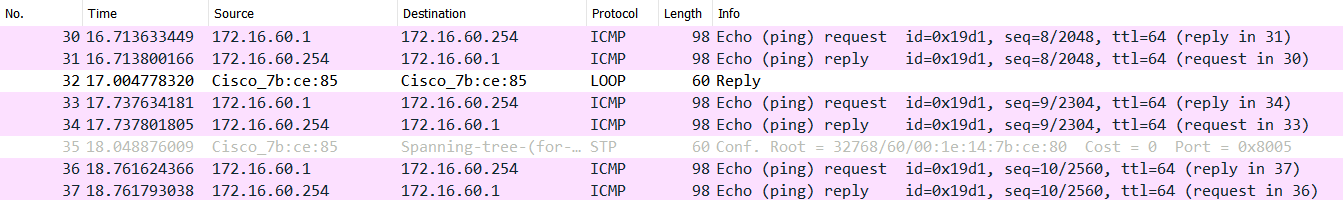
\includegraphics[scale=0.55]{exp3-step6-ping-60.254-from-gnu63.png}
\caption{Ping 172.16.60.254 a partir do gnu63}
\end{figure}

\begin{figure}[h]
	\centering
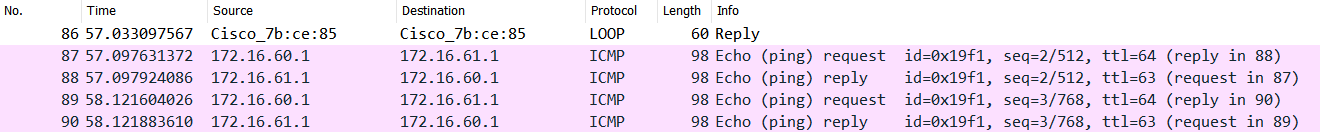
\includegraphics[scale=0.55]{exp3-step6-ping-61.1-from-gnu63.png}
\caption{Ping 172.16.61.1 a partir do gnu63}
\end{figure}

\begin{figure}[h]
	\centering
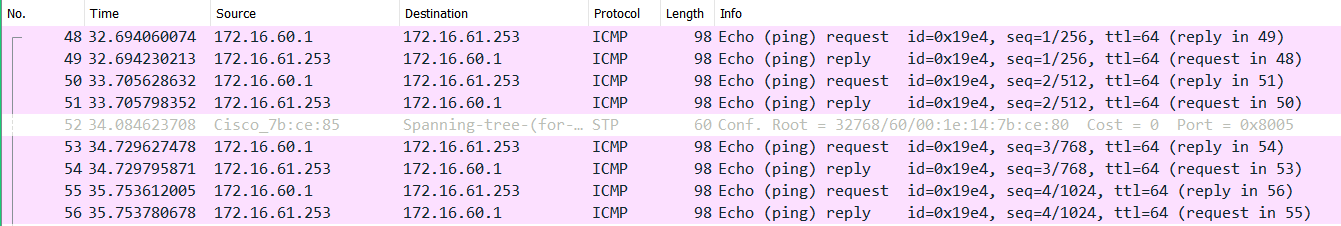
\includegraphics[scale=0.55]{exp3-step6-ping-61.253-from-gnu63.png}
\caption{Ping 172.16.61.253 a partir do gnu63}
\end{figure}

\newpage
\begin{figure}[h]
	\centering
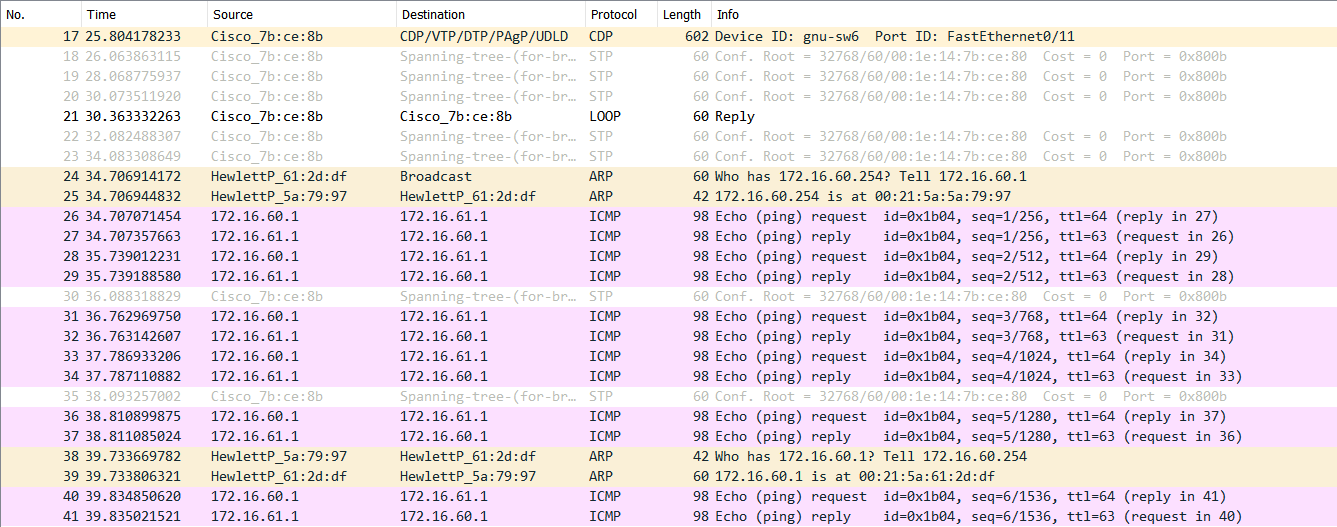
\includegraphics[scale=0.60]{exp3-step10-ping-gnu62-from-gnu63-eth0.png}
\caption{Ping do gnu63 para gnu62 e capturar no eth0 do gnu64}
\end{figure}

\begin{figure}[h]
	\centering
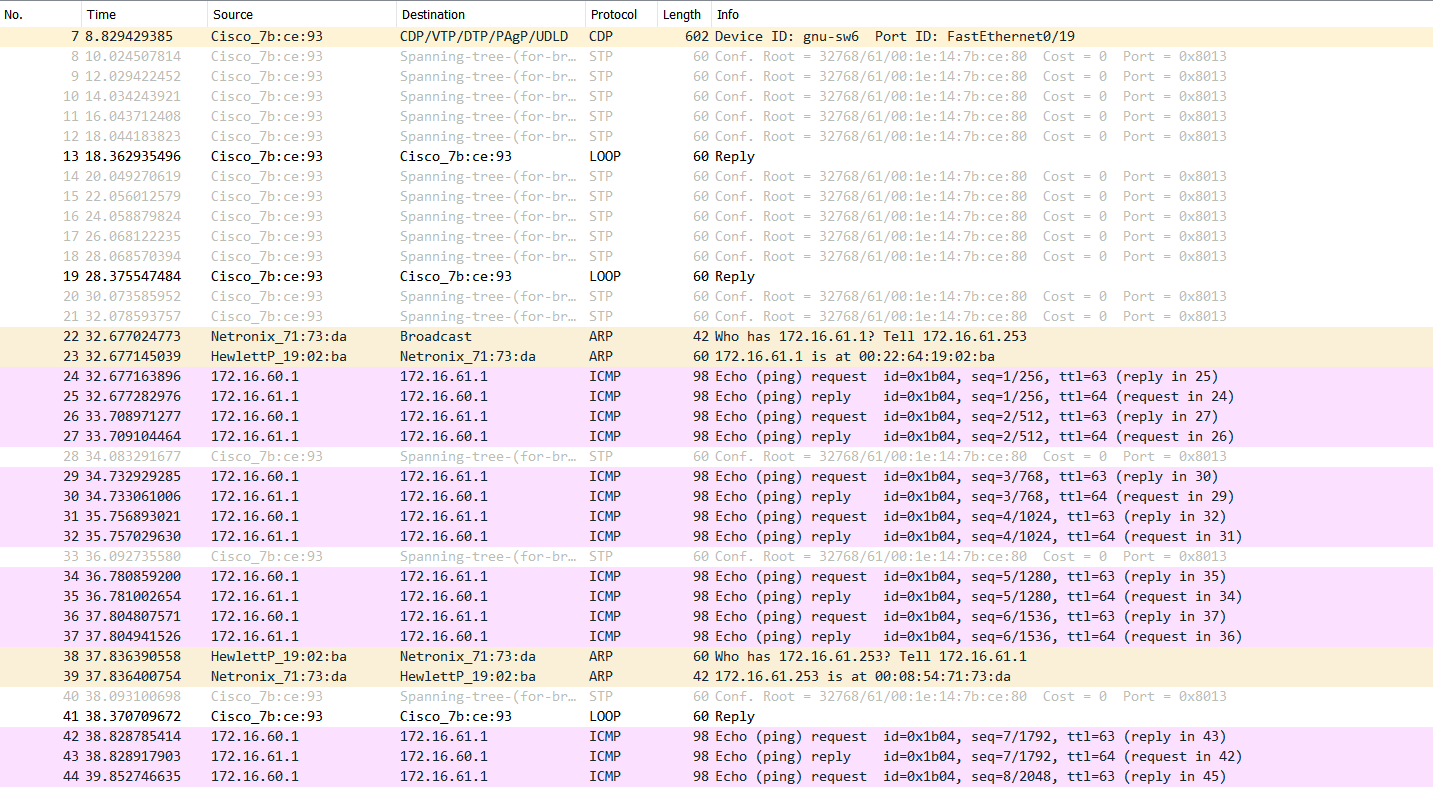
\includegraphics[scale=0.55]{exp3-step10-ping-gnu62-from-gnu63-eth1.png}
\caption{Ping do gnu63 para gnu62 e capturar no eth1 do gnu64}
\end{figure}

\newpage
\subsection{Experiência 4}
\begin{figure}[h]
	\centering
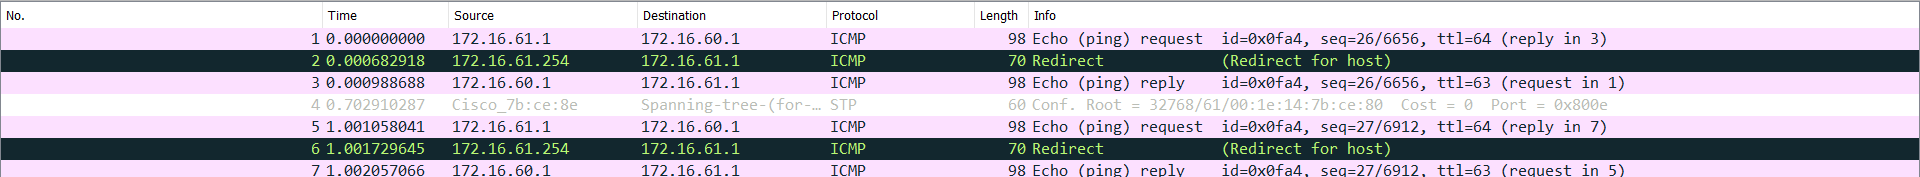
\includegraphics[scale=0.40]{exp4-step4-ping-gnu63-from-gnu62.png}
\caption{Ping do GNU62 para GNU63 sem rota para GNU64 e com redirecionamento}
\end{figure}

\begin{figure}[h]
	\centering
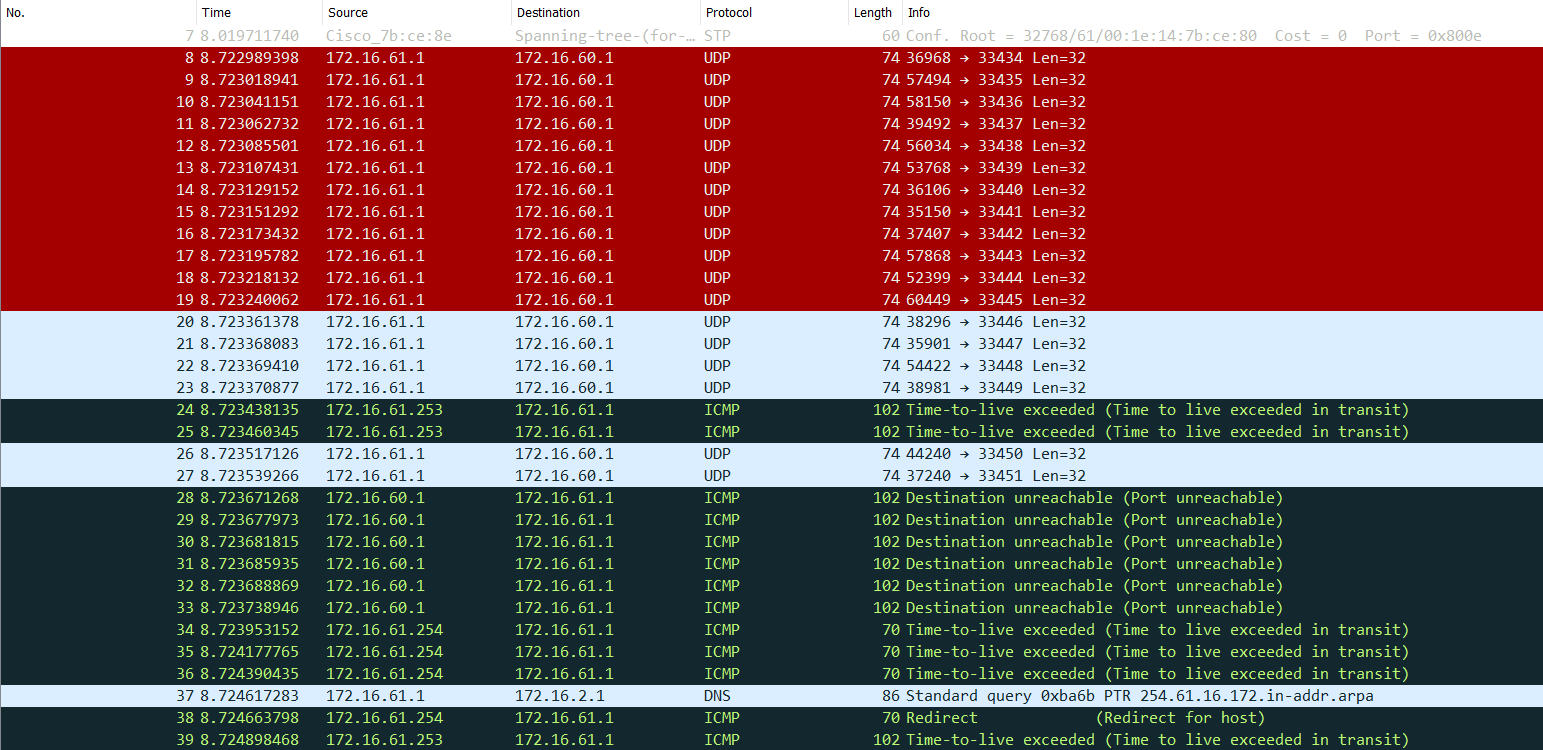
\includegraphics[scale=0.50]{exp4-traceroute.png}
\caption{Traceroute}
\end{figure}

\begin{figure}[h]
	\centering
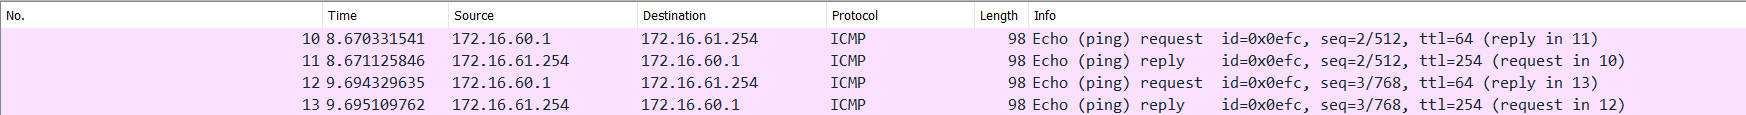
\includegraphics[scale=0.43]{exp4-step7.png}
\caption{Ping do GNU63 para o router com NAT}
\end{figure}

\subsection{Experiência 5}
\begin{figure}[h]
	\centering
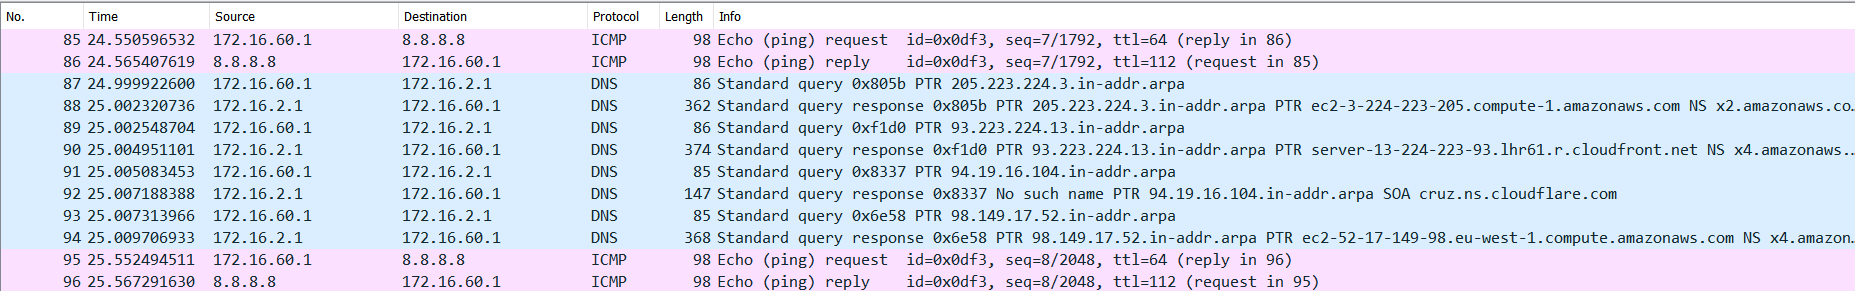
\includegraphics[scale=0.40]{exp5-step3.png}
\caption{Ping 8.8.8.8}
\end{figure}

\newpage
\subsection{Experiência 6}
\begin{figure}[h]
	\centering
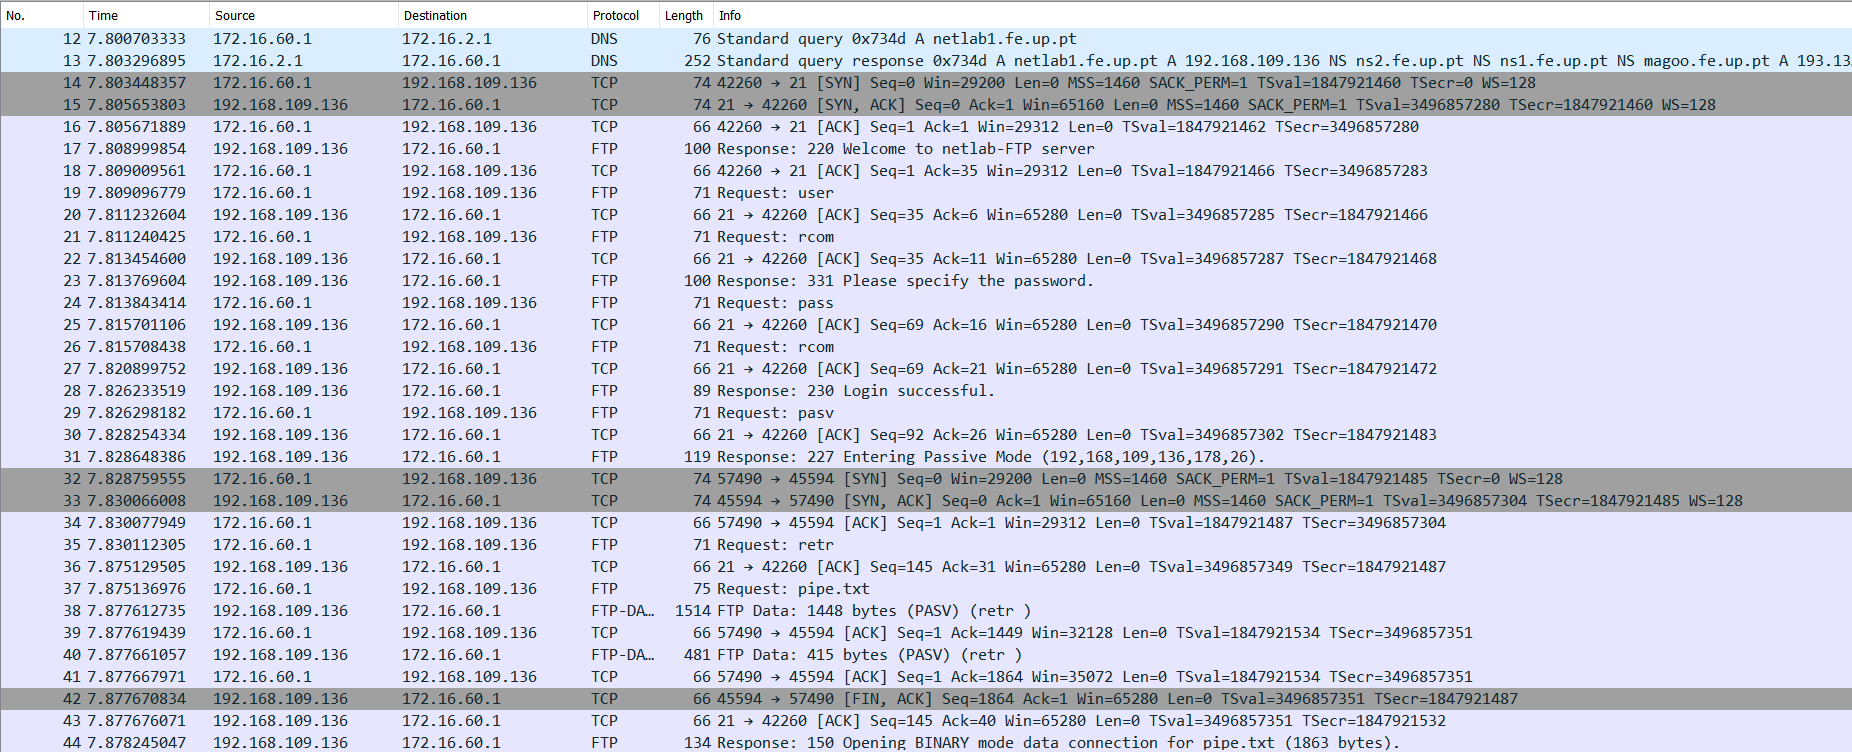
\includegraphics[scale=0.37]{exp6-step3-part1.png}
\caption{FTP download - Part 1}
\end{figure}

\begin{figure}[h]
	\centering
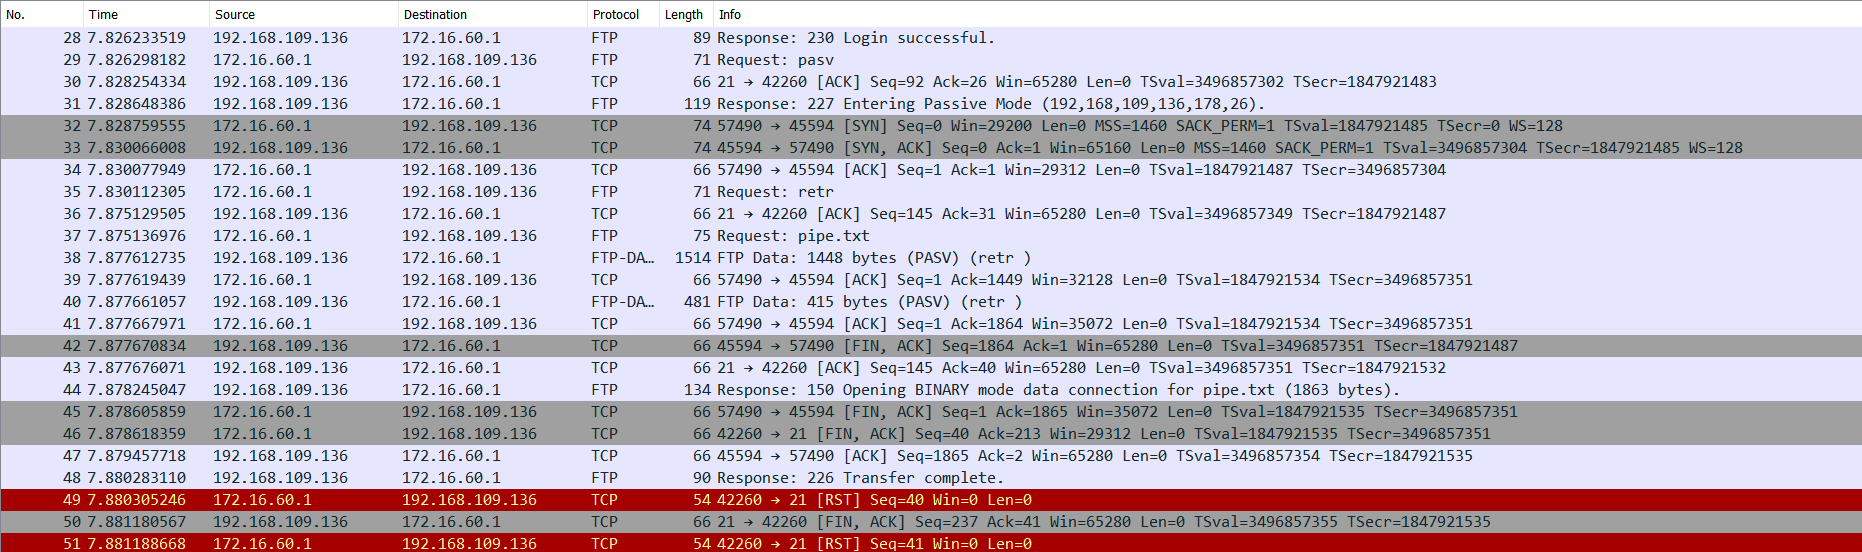
\includegraphics[scale=0.37]{exp6-step3-part2.png}
\caption{FTP download - Part 2}
\end{figure}

\begin{figure}[h]
	\centering
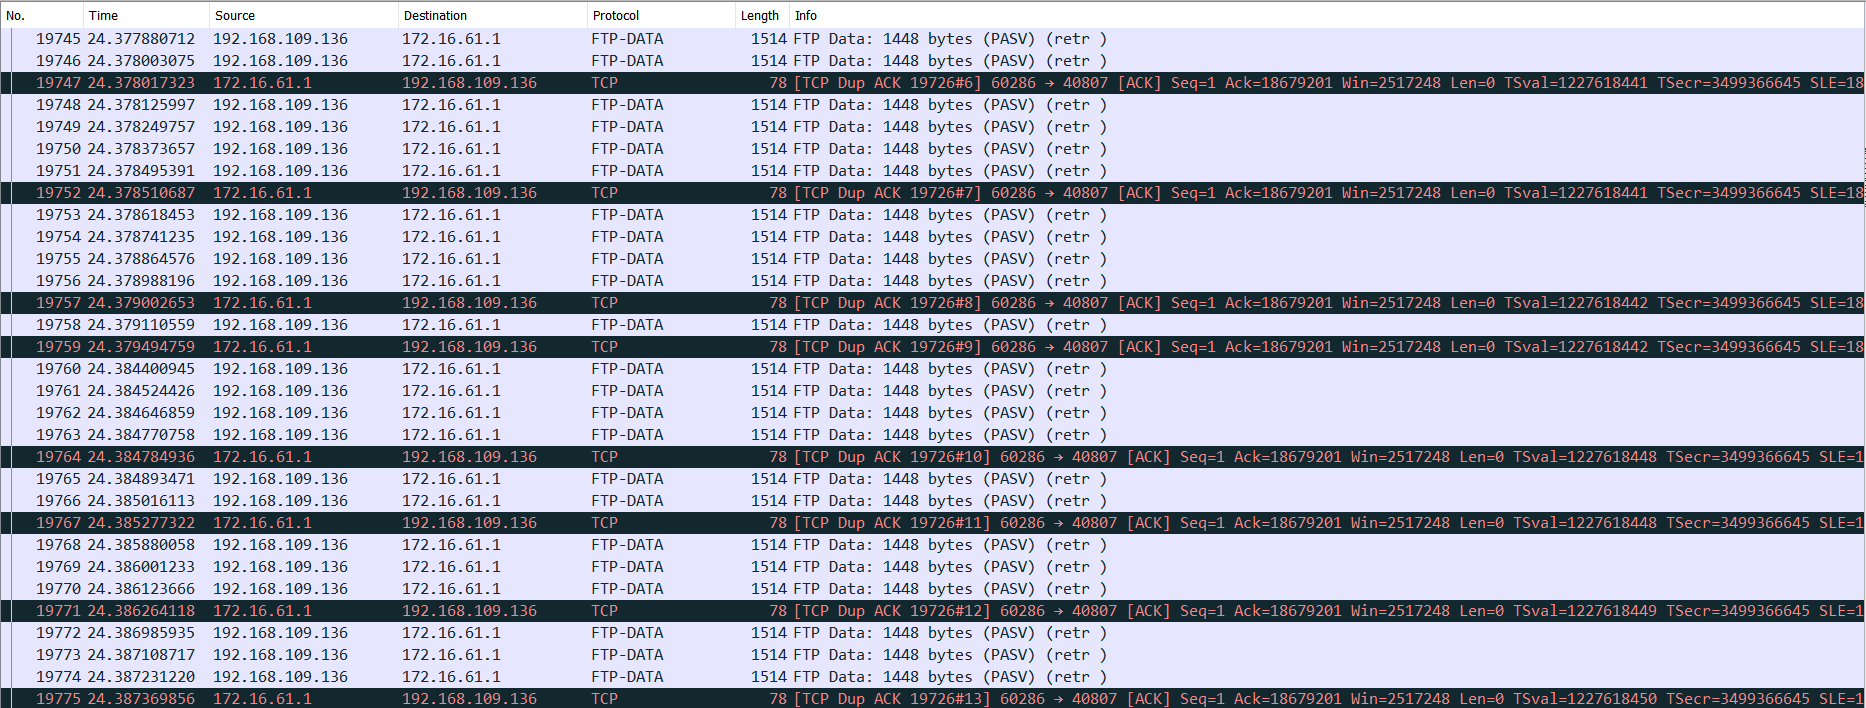
\includegraphics[scale=0.37]{exp6-step5-error.png}
\caption{DUP ACK durante a transferência}
\end{figure}

\newpage
\begin{figure}[h]
	\centering
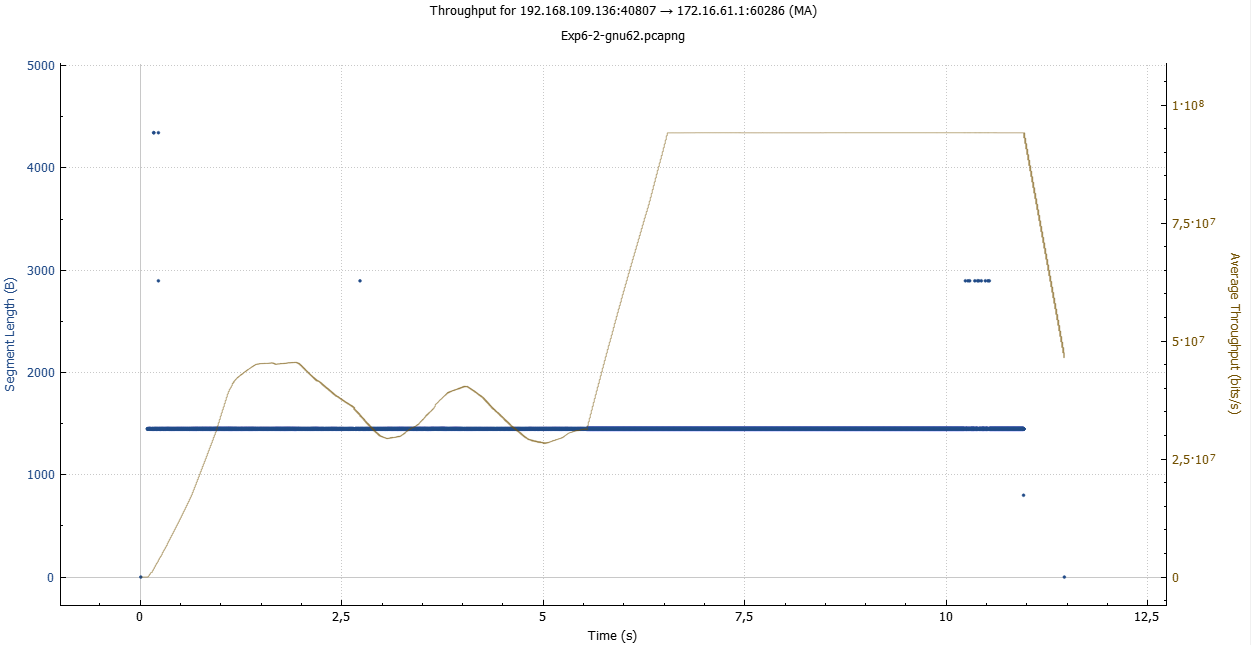
\includegraphics[scale=0.35]{exp6-step5-gnu62-graph.png}
\caption{Taxa de transferência no gnu62}
\end{figure}

\begin{figure}[h]
	\centering
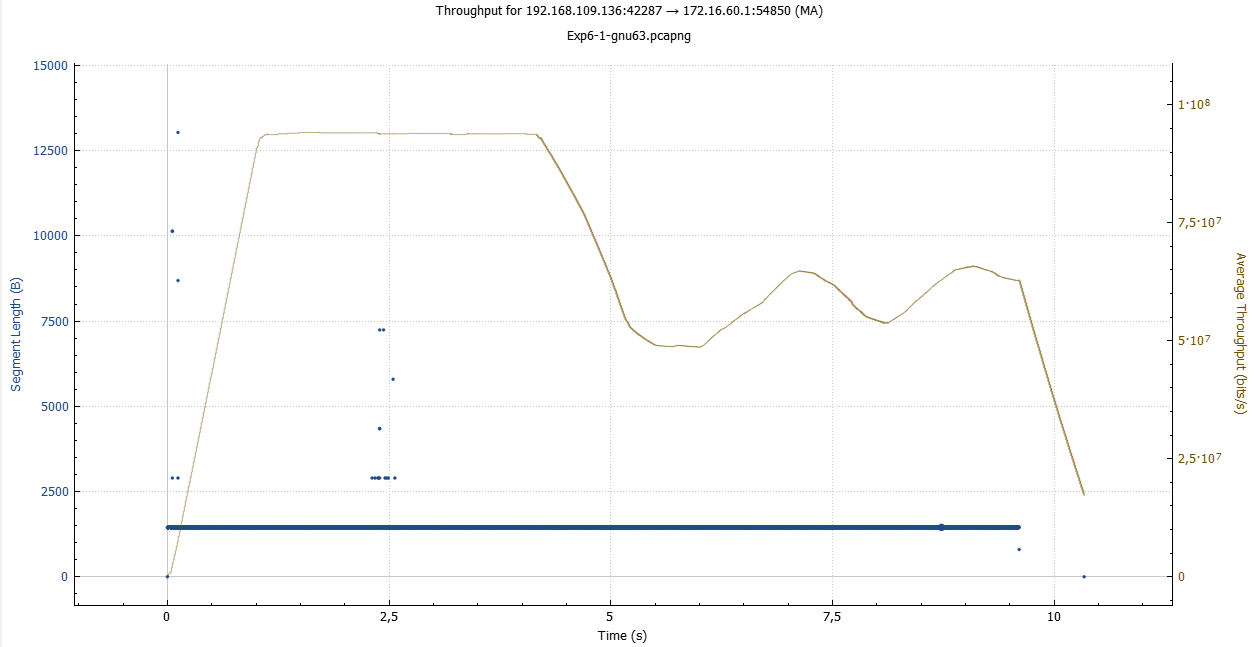
\includegraphics[scale=0.35]{exp6-step5-gnu63-graph.png}
\caption{Taxa de transferência no gnu63}
\end{figure}

\newpage
\section{Anexo II - Outras Imagens}
\begin{figure}[h]
	\centering
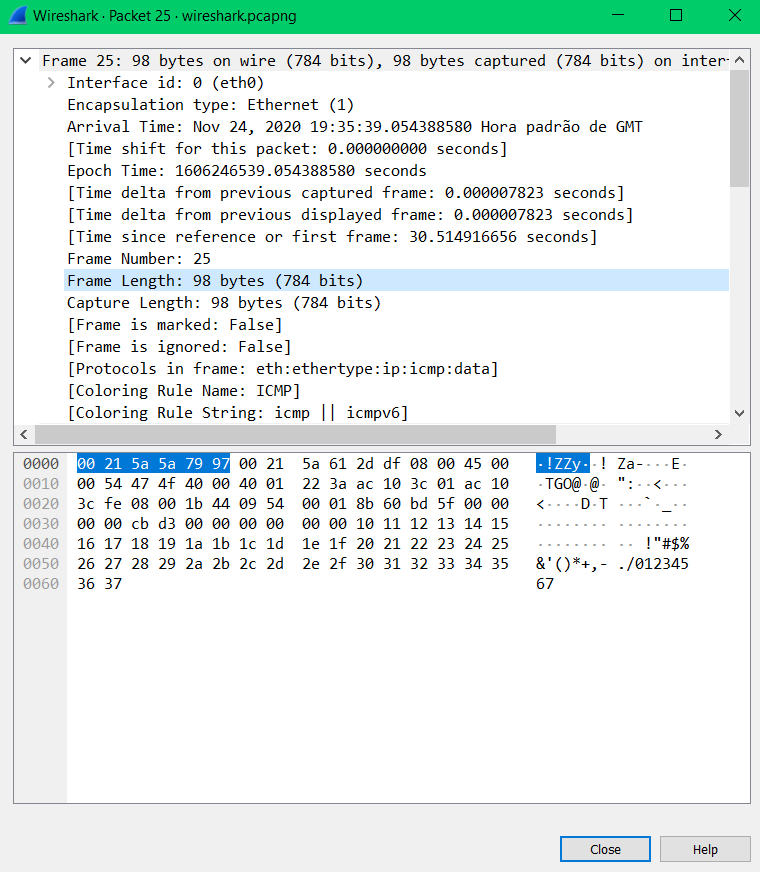
\includegraphics[scale=0.30]{package-length.png}
\caption{Package Lenght}
\end{figure}

\begin{figure}[h]
	\centering
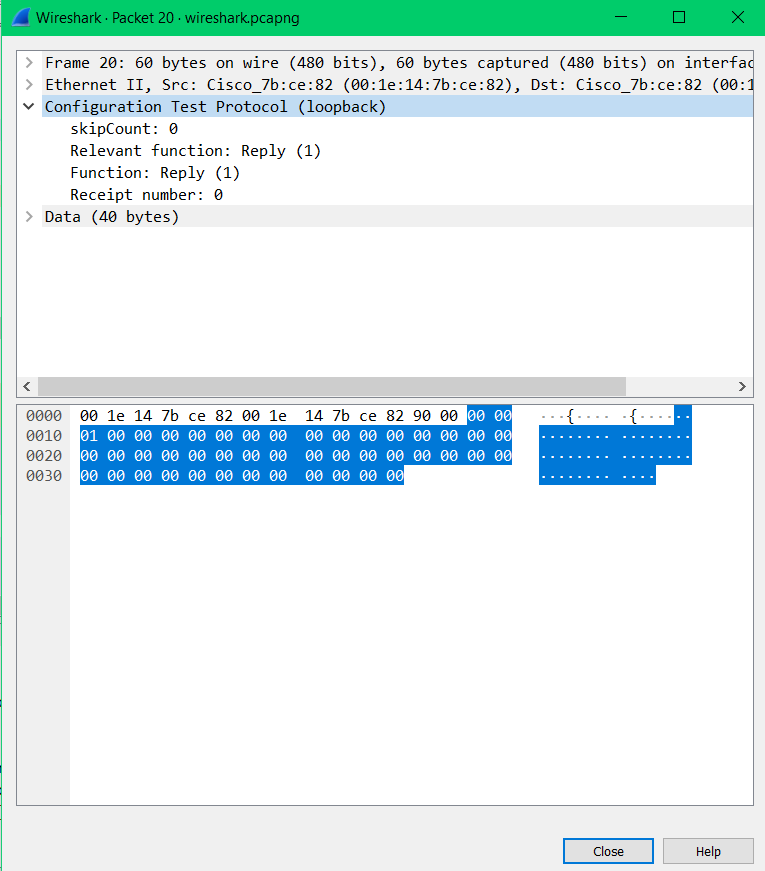
\includegraphics[scale=0.30]{loopback.png}
\caption{LOOP}
\end{figure}

\begin{figure}[h]
	\centering
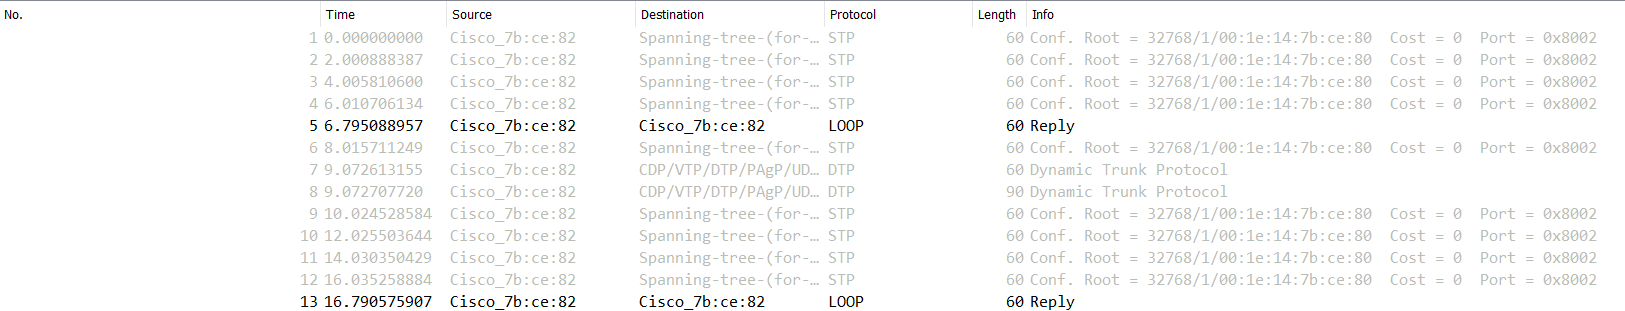
\includegraphics[scale=0.45]{loopback-2.png}
\caption{LOOP}
\end{figure}

\newpage
\subsection{Configuração do NAT}
\begin{lstlisting}
	# Configurar a interface interna do router
	conf t 
	interface fastethernet 0/0
	ip address 172.16.y1.254 255.255.255.0 
	no shutdown 
	ip nat inside 
	exit 
	
	# Configurar a interface externa do router
	interface fastethernet 0/1
	ip address 172.16.2.y9 255.255.255.0 
	no shutdown 
	ip nat outside 
	exit 
	
	# NAT
	ip nat pool ovrld 172.16.2.y9 172.16.2.y9 prefix 24 
	ip nat inside source list 1 pool ovrld overload 
	
	# Lista de acesso
	access-list 1 permit 172.16.y0.0 0.0.0.7 
	access-list 1 permit 172.16.y1.0 0.0.0.7 
	
	# Rotas
	ip route 0.0.0.0 0.0.0.0 172.16.2.254 
	ip route 172.16.y0.0 255.255.255.0 172.16.y1.253 
\end{lstlisting}

\newpage
\section{Anexo III - Código}
\subsubsection{utils.h}
\begin{lstlisting}
	struct hostent;

	enum code_state {start, first_digit, second_digit, third_digit, last_line, code_received};
	
	enum pasv_state {pasv_start, h1, h2, h3, h4, p1, p2, pasv_end};
	
	int parseArguments(char* argument, char* user, char* pass, char* host, char* file_path);
	
	struct hostent* getIP(char *host);
	
	void readServerResponse(int sockfd, char *response, char *fullResponse);
	
	int login(int sockfd, char *user, char *pass);
	
	int activatePassiveMode(int sockfd);
	
	int download_file(int sockfd, int sockfd_client, char* file_path);
\end{lstlisting}

\subsubsection{utils.c}
\begin{lstlisting}
	#include <stdio.h>
	#include <stdlib.h>
	#include <unistd.h>
	#include <string.h>
	#include <errno.h> 
	#include <netdb.h> 
	#include <sys/types.h>
	#include <netinet/in.h> 
	#include <arpa/inet.h>
	#include <ctype.h>
	#include <libgen.h>
	
	#include "utils.h"
	
	#define BUFFER_SIZE 1024
	
	int parseArguments(char* argument, char* user, char* pass, char* host, char* file_path) {
	
	  // Parse the initial part of the argument: "ftp://"
	  if(strncmp(argument, "ftp://", 6) != 0) {
		fprintf(stderr,"Invalid Argument: it should start with 'ftp://'\n");
			return -1;
	  }
	
	  int i = 6, j;
	
	  if(strchr(argument, '@') != NULL) {   // User and pass present in input
		// Parse the part of the argument relative to the user
		while (argument[i] != ':') {
		  user[i - 6] = argument[i];
		  i++;
		}
		user[i - 6] = '\0';
	
		// Parse the part of the argument relative to the pass
		i++;
		j = i;
		while (argument[j] != '@') {
		  pass[j - i] = argument[j];
		  j++;
		}
		pass[j - i] = '\0';
		j++;
	  }
	  else {
		user[0] = '\0';
		pass[0] = '\0';
		j = 6;
	  }
	
	  // Parse the part of the argument relative to the host
	  int k = j;
	  while (argument[k] != '/') {
		host[k - j] = argument[k];
		k++;
	  }
	  host[k - j] = '\0';
	
	  // Parse the part of the argument relative to the url path
	  k++;
	  int l = k;
	  while (argument[l] != '\0') {
		file_path[l - k] = argument[l];
		l++;
	  }
	  file_path[l - k] = '\0';
	
	  return 0;
	}
	
	struct hostent* getIP(char *host) {
		struct hostent *h;
	
	  /*
	  struct hostent {
		  char    *h_name;	Official name of the host. 
		  char    **h_aliases;	A NULL-terminated array of alternate names for the host. 
		  int     h_addrtype;	The type of address being returned; usually AF_INET.
		  int     h_length;	The length of the address in bytes.
		  char    **h_addr_list;	A zero-terminated array of network addresses for the host. 
		  Host addresses are in Network Byte Order. 
	  };
	
	  #define h_addr h_addr_list[0]	The first address in h_addr_list. 
	  */
	
	  if ((h=gethostbyname(host)) == NULL) {  
		herror("gethostbyname");
		return NULL;
	  }
	
	  return h;
	}
	
	void readServerResponse(int sockfd, char *response, char *fullResponse) {
	  enum code_state state = start;
	  char character;
	  int i = 0;
	
	  while(state != code_received) {
		read(sockfd, &character, 1);
	
		fullResponse[i] = character;
		i++;
	
		switch(state) {
		  case start:
			if (isdigit(character)) {
			  state = first_digit;
			  response[0] = character;
			}
			break;
		  case first_digit:
			if (isdigit(character)) {
			  state = second_digit;
			  response[1] = character;
			}
			else {
			  state = start;
			  memset(response,0,sizeof(response));
			}
			break;
		  case second_digit:
			if (isdigit(character)) {
			  state = third_digit;
			  response[2] = character;
			}
			else {
			  state = start;
			  memset(response,0,sizeof(response));
			}
			break;
		  case third_digit:
			if ((character == ' ')) {
			  state = last_line;
			}
			else {
			  state = start;
			  memset(response,0,sizeof(response));
			}
			break;
		  case last_line:
			if ((character == '\n')) {
			  state = code_received;
			}
			break;
		}
	  }
	
	  fullResponse[i] = '\0';
	  printf("\nServer Response:\n%s\n", fullResponse);
	}
	
	int login(int sockfd, char *user, char *pass) {
	  printf(">> Sending username...\n");
	
	  // Send username
		write(sockfd, "user ", 5);
	  write(sockfd, user, strlen(user));
	  write(sockfd, "\n", 1);
	
	  char response[3];
	  char fullResponse[1024];
	
	  readServerResponse(sockfd, response, fullResponse);
	
	  while(response[0] == '4') {
		// Resend username
		write(sockfd, "user ", 5);
		write(sockfd, user, strlen(user));
		write(sockfd, "\n", 1);
			readServerResponse(sockfd, response, fullResponse);
	  }
	
	  if (response[0] == '2') {   // Password not requested - Login successful
		return 0;
	  }
	
	  if(response[0] != '3') {
		fprintf(stderr,"Username not accepted\n");
			return -1;
	  }
	
	  printf(">> Sending password...\n");
	
	  // Send pass
		write(sockfd, "pass ", 5);
	  write(sockfd, pass, strlen(pass));
	  write(sockfd, "\n", 1);
	
	  memset(response,0,sizeof(response));
	  memset(fullResponse,0,sizeof(fullResponse));
	  readServerResponse(sockfd, response, fullResponse);
	
	  while(response[0] == '4') {
		// Resend pass
		write(sockfd, "pass ", 5);
		write(sockfd, pass, strlen(pass));
		write(sockfd, "\n", 1);
			readServerResponse(sockfd, response, fullResponse);
	  }
	
	  if(strncmp(response, "230", 3) != 0) {
		fprintf(stderr,"Password not accepted\n");
			return -2;
	  }
	
	  return 0;
	}
	
	int activatePassiveMode(int sockfd) {
	  char response[4];
	  char fullResponse[512];
	  char number[4];
	  int i = 0;
	  int pasv_numbers[6];
	  int j = 0;
	  int k = 0;
	
	  write(sockfd, "pasv\n", 5);
	
	  enum pasv_state state = pasv_start;
	  char character;
	
	  memset(fullResponse,0,sizeof(fullResponse));
	
	  while(state != pasv_end) {
		read(sockfd, &character, 1);
		fullResponse[k] = character;
		k++;
	
		switch(state) {
		  case pasv_start:
			if (character == '(') {
			  state = h1;
			  memset(number,0,sizeof(number));
			}
			break;
		  case h1:
			if (isdigit(character)) {
			  number[i] = character;
			  i++;
			}
			else if (character == ',') {
			  state = h2;
			  number[3] = '\0';
			  pasv_numbers[j] = atoi(number);
			  memset(number,0,sizeof(number));
			  i = 0;
			  j++;
			}
			break;
		  case h2:
			if (isdigit(character)) {
			  number[i] = character;
			  i++;
			}
			else if (character == ',') {
			  state = h3;
			  number[3] = '\0';
			  pasv_numbers[j] = atoi(number);
			  memset(number,0,sizeof(number));
			  i = 0;
			  j++;
			}
			break;
		  case h3:
			if (isdigit(character)) {
			  number[i] = character;
			  i++;
			}
			else if (character == ',') {
			  state = h4;
			  number[3] = '\0';
			  pasv_numbers[j] = atoi(number);
			  memset(number,0,sizeof(number));
			  i = 0;
			  j++;
			}
			break;
		  case h4:
			if (isdigit(character)) {
			  number[i] = character;
			  i++;
			}
			else if (character == ',') {
			  state = p1;
			  number[3] = '\0';
			  pasv_numbers[j] = atoi(number);
			  memset(number,0,sizeof(number));
			  i = 0;
			  j++;
			}
			break;
		  case p1:
			if (isdigit(character)) {
			  number[i] = character;
			  i++;
			}
			else if (character == ',') {
			  state = p2;
			  number[3] = '\0';
			  pasv_numbers[j] = atoi(number);
			  memset(number,0,sizeof(number));
			  i = 0;
			  j++;
			}
			break;
		  case p2:
			if (isdigit(character)) {
			  number[i] = character;
			  i++;
			}
			else if (character == '\n') {
			  state = pasv_end;
			  number[3] = '\0';
			  pasv_numbers[j] = atoi(number);
			}
			break;
		}
	  }
	
	  int port = pasv_numbers[4]*256 + pasv_numbers[5];
	
	  fullResponse[k] = '\0';
	  printf("Server Response: \n%s\n", fullResponse);
	
	  return port;
	}
	
	int download_file(int sockfd, int sockfd_client, char* file_path) {
	  // Send file request
		write(sockfd, "retr ", 5);
	  write(sockfd, file_path, strlen(file_path));
	  write(sockfd, "\n", 1);
	
	  char response[3];
	  char fullResponse[1024];
	
	  readServerResponse(sockfd, response, fullResponse);
	
	  while(response[0] == '4') {
		// Resend file request
		write(sockfd, "retr ", 5);
		write(sockfd, file_path, strlen(file_path));
		write(sockfd, "\n", 1);
			readServerResponse(sockfd, response, fullResponse);
	  }
	
		if (strncmp(response, "150", 3) != 0) {
			fprintf(stderr,"Couldn't open file\n");
			return -1;
		}
	
	  char* filename;
	
	  filename = basename(file_path);
	
	  FILE *file = fopen(filename, "wb+");
	  
	  char file_part[BUFFER_SIZE];
	  int bytes_read, elems_written;
	
	  while((bytes_read = read(sockfd_client, file_part, BUFFER_SIZE)) > 0) {
		elems_written = fwrite(file_part, bytes_read, 1, file);
		if (elems_written != 1) {
		  fprintf(stderr,"Error downloading file\n");
			  return -2;
		}
	  }
	
	  fclose(file);
	
	  return 0;
	}
\end{lstlisting}

\subsubsection{clientTCP.c}
\begin{lstlisting}
	/*      (C)2000 FEUP  */

	#include <stdio.h>
	#include <sys/types.h>
	#include <sys/socket.h>
	#include <netinet/in.h>
	#include <arpa/inet.h>
	#include <stdlib.h>
	#include <unistd.h>
	#include <signal.h>
	#include <netdb.h>
	#include <string.h>
	#include <libgen.h>
	#include <sys/time.h>
	
	#include "utils.h"
	
	#define SERVER_PORT 21
	#define SERVER_ADDR "192.168.28.96"
	
	#define MAX_SIZE 256
	
	int main(int argc, char** argv){
	
		int	sockfd, sockfd_client;
		struct	sockaddr_in server_addr;
		struct	sockaddr_in server_addr_client;
	
		char user[MAX_SIZE];
		char pass[MAX_SIZE];
		char host[MAX_SIZE];
		char file_path[MAX_SIZE];
	
		struct hostent *h;
	
		if (argc != 2) {
			fprintf(stderr,"Usage: ./download ftp://[user]:[pass]@[host]/[url-path]\n");
			exit(1);
		}
	
		if (parseArguments(argv[1], user, pass, host, file_path) < 0) {
			fprintf(stderr,"Usage: ./download ftp://[user]:[pass]@[host]/[url-path]\n");
			exit(2);
		}
	
		if (user[0] == '\0' && pass[0] == '\0') {
			strcpy(user, "anonymous");
			strcpy(pass, "anypass");
		}
	
		printf("\n-------------------- INPUT DATA --------------------\n");
		printf("User: %s\nPassword: %s\nHost: %s\nURL path: %s\n", user, pass, host, file_path);
	
		if ((h = getIP(host)) == NULL) {
			fprintf(stderr,"Couldn't get Host IP\n");
			exit(3);
		}
	
		printf("\nHost name  : %s\n", h->h_name);
		printf("IP Address : %s\n",inet_ntoa(*((struct in_addr *)h->h_addr)));
		printf("----------------------------------------------------\n");
		
		/*server address handling*/
		bzero((char*)&server_addr,sizeof(server_addr));
		server_addr.sin_family = AF_INET;
		server_addr.sin_addr.s_addr = inet_addr(inet_ntoa(*((struct in_addr *)h->h_addr)));	/*32 bit Internet address network byte ordered*/
		server_addr.sin_port = htons(SERVER_PORT);		/*server TCP port must be network byte ordered */
		
		/*open an TCP socket*/
		if ((sockfd = socket(AF_INET,SOCK_STREAM,0)) < 0) {
			perror("socket()");
			exit(4);
		}
	
		/*connect to the server*/
		if(connect(sockfd, (struct sockaddr *)&server_addr, sizeof(server_addr)) < 0) {
			perror("connect()");
			exit(4);
		}
	
		char serverResponse[3];
		char fullResponse[1024];
	
		printf("\n>> Conecting to the server...\n");
	
		readServerResponse(sockfd, serverResponse, fullResponse);
	
		if (strncmp(serverResponse, "220", 3) != 0) {
			fprintf(stderr,"Connection lost\n");
			exit(5);
		}
	
		if (login(sockfd, user, pass) < 0) {
			fprintf(stderr,"Couldn't login\n");
			exit(6);
		}
	
		printf(">> Entering passive mode...\n\n");
	
		int port;
		if ((port = activatePassiveMode(sockfd)) < 0) {
			fprintf(stderr,"Couldn't enter passive mode\n");
			exit(7);
		}
	
		printf(">> Connecting to the client port...\n");
	
		/*server address handling*/
		bzero((char*)&server_addr_client,sizeof(server_addr_client));
		server_addr_client.sin_family = AF_INET;
		server_addr_client.sin_addr.s_addr = inet_addr(inet_ntoa(*((struct in_addr *)h->h_addr)));	/*32 bit Internet address network byte ordered*/
		server_addr_client.sin_port = htons(port);		/*server TCP port must be network byte ordered */
		
		/*open an TCP socket*/
		if ((sockfd_client = socket(AF_INET,SOCK_STREAM,0)) < 0) {
			perror("socket()");
			exit(4);
		}
	
		/*connect to the server*/
		if(connect(sockfd_client, (struct sockaddr *)&server_addr_client, sizeof(server_addr_client)) < 0) {
			perror("connect()");
			exit(4);
		}
	
		printf("<< Client connection successful\n\n");
	
		printf(">> Starting downloading the file\n");
	
		struct timeval init_time;
		struct timeval current_time;
		gettimeofday(&init_time, 0);
	
		if (download_file(sockfd, sockfd_client, file_path) < 0) {
			fprintf(stderr,"Couldn't download file\n");
			exit(8);
		}
	
		gettimeofday(&current_time, 0);
		double elapsedTime = (current_time.tv_usec - init_time.tv_usec) / 1000.0 +
						(current_time.tv_sec - init_time.tv_sec) * 1000.0;
	
		char *filename = basename(file_path);
	
		printf("File %s downloaded successfully in %f seconds!\n", filename, elapsedTime/1000.0);
	
		if (close(sockfd_client) < 0) {
			perror("Error closing client socket");
			exit(9);
		}
	
		if (close(sockfd)) {
			perror("Error closing server socket");
			exit(9);
		}
	
		exit(0);
	}
\end{lstlisting}

\end{document}

